\chapter{Problèmes rencontrés} \label{problemes}
Comme dans chaque projet, un ensemble de problèmes se sont produits. Dans ce chapitre se trouve la description de chaque problème majeur rencontré.

\section*{Utilisation du Kinect en passant par NodeJS}  \label{probNodeKinect}
A la fin du projet de semestre, un projet \textit{GitHub} Node Kinect \cite{NodeKinect} a été trouvé. Il permet de capturer les données du \textit{Kinect} directement avec \textit{NodeJS}, donc de ne pas utiliser \textit{Visual Studio} et d'avoir un projet entièrement en \textsf{JavaScript}. \\ 

Le projet \textit{Node Kinect} utilise les outils suivants :
\begin{itemize}
\item La librairie \textit{Libusb} est une libraire C, open source, qui donne accès aux périphériques USB sur beaucoup de systèmes d'exploitation (pour plus d'information voir \cite{libusb}).\\ 
Elle permet de communiquer avec le \textit{Kinect}. 
\item Le driver \textit{Libfreenect} est un driver implémenté par \textit{OpenKinect}. \textit{OpenKinect} est une communauté open source de personnes qui veulent faire fonctionner le \textit{Kinect} avec d'autres systèmes d'exploitation que Windows (pour plus d'informations sur \textit{Libfreenect}~\cite{libfreenect} ou sur OpenKinect~\cite{OpenKinect}).  \\
Ce driver permet de capturer les données du \textit{Kinect} et donc de substituer le \textit{Kinect SDK}. \\

\end{itemize}

Lors de l'installation de \textit{Libfreenect} et de l'installation des logiciels nécessaires à son fonctionnement, des erreurs apparaissaient car plusieurs logiciels ou librairies manquaient. Après plus d'une semaine bloquée sur cette installation et donc dans l'incapacité de commencer à utiliser le \textit{Kinect}, l'utilisation du projet \textit{Node Kinect} a été abandonnée. Finalement, la gestion du \textit{Kinect} dans \textit{Virtual-Vertigo} s'est faite avec le \textit{Kinect SDK 1.8, Visual Studio et C\#} \. L'envoi des données capturées passe par un serveur Web.

%%%%%%%%%%%%%%%%%%%%%%%%%%%%%%%%%%%%%%%%%%%%%%%%%%%%%%%%%%%%%%%%%%%%%%%%%%%%%%%%%%%%%%%%%%%%%%%%%%%%%%%%%%%%%%%%%%%%%%%%%%%
\section*{Utilisation KinectHTML5 sur un site sécurisé}  \label{probKinectHTML5}
Toujours durant le travail de semestre, le projet \textit{Visual Studio KinectHTML5} \cite{KinectHTML5} a été trouvé. Ce projet permet de capturer des données du \textit{Kinect} et de les envoyer via les \textit{WebSockets} à un client HTML5. Il a été choisi car il correspondait aux besoins du projet \textit{Virtual-Vertigo}. Le projet \textit{KinectHTML5} est constitué de deux parties :
\begin{enumerate}
\item un projet client dans lequel se trouve la page HTML5 et les scripts nécessaires à la connexion aux \textit{WebSockets}, à la récupération des données du \textit{Kinect} et l'affichage des informations captées sur un canvas;
\item un projet serveur sur lequel s'exécute le serveur \textit{WebSocket} et où se font la capture et l'envoi des données.\\

\end{enumerate}

En utilisant ce projet localement tout fonctionnait parfaitement. Cependant, lors de l'intégration de ce projet au serveur d'hébergement, ça ne fonctionnait plus. En effet, \textit{KinectHTML5} utilise des \textit{WebSockets} tandis que le serveur d'hébergement utilise HTTPS. Pour que le projet fonctionne, il fallait l'adapter pour utiliser des \textit{WebSockets} sécurisés. Mais les \textit{WebSockets} sécurisés nécessitent un certificat. Celui-ci a alors été créé mais il a été impossible de l'ajouter au serveur d'hébergement. \\

La solution a été d'utiliser un \textit{serveur NodeJS} avec \textit{Socket.io} servant de pont entre les clients HTML et le \textit{Kinect}. Après quelques recherches, le \textit{projet Visual Studio SocketIOC\# Client} a été trouvé. Il permet à un programme C\# de se connecter à un \textit{serveur NodeJS} utilisant \textit{Socket.io} (pour plus d'informations sur le projet \textit{SocketIOC\#} voir \cite{SocketIOCSharp} ou sur \textit{Socket.io} \cite{SocketIO}).

%%%%%%%%%%%%%%%%%%%%%%%%%%%%%%%%%%%%%%%%%%%%%%%%%%%%%%%%%%%%%%%%%%%%%%%%%%%%%%%%%%%%%%%%%%%%%%%%%%%%%%%%%%%%%%%%%%%%%%%%%%%

\section*{Animation du personnage - mapping squelette kinect et squelette blender}  \label{probSquelette}

Lorsque le personnage virtuel 3D a été créé avec \textit{MakeHuman}, un squelette a été ajouté au personnage afin de pouvoir l'animer. Pour une animation la plus réaliste possible, l'idée de mapper le squelette du \textit{Kinect} et le squelette présent dans le personnage 3D est apparu. Cependant, après quelques recherches et tests, il était impossible de mapper les deux squelettes. En effet, lorsque le personnage est exporté en format X3D avec \textit{Blender}, le personnage devient rigide. Il est impossible d'accéder à chaque membre du squelette dans le personnage.\\

La solution mise en place favorise l'animation des membres au dépend du réalisme du personnage 3D. Le squelette de la personne a été reconstruit en 3D directement sur \textit{X3DOM}. En utilisant les données reçues, cela a permis d'animer les membres du personnage. L'animation des membres a été effectuée en calculant l'angle entre les articulations reliées. Cet angle permet de savoir comment effectuer la rotation du membre.

%%%%%%%%%%%%%%%%%%%%%%%%%%%%%%%%%%%%%%%%%%%%%%%%%%%%%%%%%%%%%%%%%%%%%%%%%%%%%%%%%%%%%%%%%%%%%%%%%%%%%%%%%%%%%%%%%%%%%%%%%%%

\section*{Animation du personnage - calcul de l'angle}  \label{probAngle}

Comme mentionné dans la section précédente, un angle a été calculé entre les articulations reliées. L'angle a été calculé, considérant chaque articulation comme un point dans l'espace. Le calcul de l'angle entre deux points est impossible. Nous avons donc calculé un troisième point avec les coordonnées des deux autres points afin de créer un triangle rectangle.\\

\begin{figure}[H]
	\centering
   		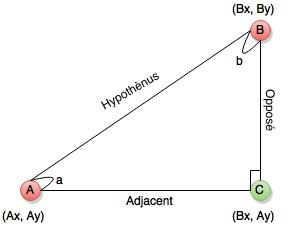
\includegraphics[scale=0.7]{Triangle.jpg}
   \caption{\label{triangle rectangle} Illustration du triangle rectangle}
\end{figure}
Sur l'illustration~\ref{triangle rectangle}, les deux points correspondant aux articulations sont en rouge, le troisième point étant en vert (une combinaison des deux autres points). En traçant les droites entre chaque point, il est possible de créer un triangle rectangle. Il permet d'utiliser les formules trigonométriques, telles que le calcul de la distance entre deux points et le calcul des angles dans un triangle rectangle. \\

Les formules de calcul de distance entre deux points appliquées sur ce triangle sont les suivantes : \\
\begin{equation}
AC = \sqrt{(B_x - A_x)^2 + (A_y - A_y)^2}
\end{equation}
\begin{equation}
BC = \sqrt{(B_x - B_x)^2 + (A_y - B_y)^2} 
\end{equation}
\begin{equation}
AB = \sqrt{(B_x - A_x)^2 + (B_y - A_y)^2} 
\end{equation}
où $A=(A_x,A_y)$, $B=(B_x,B_y)$ et $C=(B_x,A_y)$

Les formules de calcul de l'angle appliquées sur ce triangle sont les suivantes : \\
\begin{equation}
b = \mathrm{acos}{(BC/AB)}
\end{equation}
\begin{equation}
a = \mathrm{asin}{(AC/AB)}
\end{equation}

Cependant, en effectuant l'implémentation de ces calculs, ceux-ci n'étaient pas assez précis et trop lents, parce que la disposition des articulations n'a pas été prise en compte. Les membres ne se déplaçaient pas comme ils le devaient. Finalement, le calcul de l'angle a été effectué en utilisant la fonction atan2 décrite à la section~\ref{atan2}. L'utilisation de cette fonction a rendu l'animation des membres plus précise et dynamique.

%%%%%%%%%%%%%%%%%%%%%%%%%%%%%%%%%%%%%%%%%%%%%%%%%%%%%%%%%%%%%%%%%%%%%%%%%%%%%%%%%%%%%%%%%%%%%%%%%%%%%%%%%%%%%%%%%%%%%%%%%%%
\pagebreak
\section*{Des données captées à la réalité}  \label{probRealite}
Lors du développement, nous avons réalisé que le \textit{Kinect} ne transmettait pas les données qu'il capte en fonction de la réalité. En effet, le \textit{Kinect} transmettait les données en fonction de son angle de vue conique. En effet l'utilisation d'un objet \texttt{CoordinateMapper} ne renvoyait pas les dimensions réelles de la personne. Pour remédier à ce problème, des mesures ont été effectuées sur un rectangle délimité :
\begin{figure}[H]
	\centering
		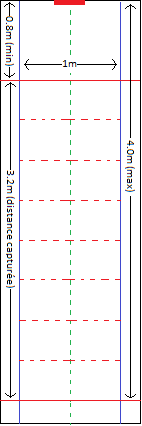
\includegraphics[scale=1]{RectangleMesures.png}
	\caption{\label{rectangleMesures} Rectangle créé sur le sol afin d'effectuer les mesures}
\end{figure}

Ces mesures ont été réalisées tous les 40 centimètres au centre du rectangle. Les points de repères suivants ont été définis :
\begin{itemize}
\item pour la distance entre deux articulations, le centre des épaules et la colonne vertébrale
\item pour l'axe x, la main posée sur une table à 3 endroits différents afin ne pas fausser les mesures entre chaque déplacement
\item pour z, les 2 pieds placés après les lignes tracées au sol \\

\end{itemize}

Voici les résultats obtenus : 
\begin{center}
	\begin{tabular}{|*{6}{c|}}
	\hline
		\textbf{Z} & \textbf{Distance} & \textbf{Z Kinect} & \textbf{Coin gauche} & \textbf{Milieu} & \textbf{Coin droit}  \\ \hline
		0.80 & 169 & 0.85 & 44 & 276 & 475\\ \hline
		1.20 & 147 & 1.25 & 72 & 271 & 447\\ \hline
		1.60 & 112 & 1.65 & 105 & 294 & 420\\ \hline
		2.00 & 92 & 2.05 & 134 & 274 & 397\\ \hline
		2.40 & 79 & 2.46 & 158 & 261 & 362\\ \hline
		2.80 & 69 & 2.86 & 160 & 257 & 357\\ \hline
		3.20 & 60 & 3.24 & 177 & 270 & 343\\ \hline
		3.60 & 54 & 3.65 & 183 & 257 & 334\\ \hline
		3.85 & 50 & 3.90 & 187 & 302 & 290\\ \hline
	\end{tabular}
\end{center}

En analysant ce tableau, les valeurs en z correspondent à la réalité moyennant un décalage de 0.5 cm. Cependant les valeurs mesurées en x ne correspondent pas et n'aide pas à trouver une formule pouvant être appliquée. Un graphique peut être tracé avec les valeurs des distances entre le centre des épaules et la colonne vertébrale: \\

\begin{figure}[H]
	\centering
		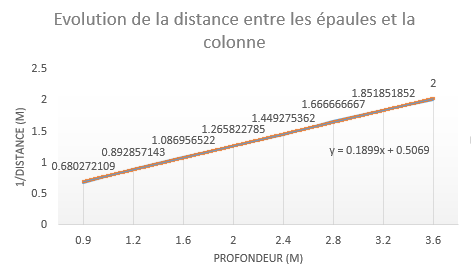
\includegraphics[scale=0.7]{evolutionDistance.png}
	\caption{\label{evolutionDistance} Évolution de la distance entre les épaules et la colonne}
\end{figure}

Finalement, le problème a été corrigé sans utiliser ces mesures. Le programme capturant les données du \textit{Kinect} a complètement été réécrit afin de capturer les données de manière absolue. En utilisant cette méthode, les valeurs en x et y capturées sont en mètres et correspondent à la réalité. 

%%%%%%%%%%%%%%%%%%%%%%%%%%%%%%%%%%%%%%%%%%%%%%%%%%%%%%%%%%%%%%%%%%%%%%%%%%%%%%%%%%%%%%%%%%%%%%%%%%%%%%%%%%%%%%%%%%%%%%%%%%%

\section*{Taille de la scène finale}  \label{taille}

Comme mentionné dans le chapitre~\ref{vertigo}, une des vues finales du projet a été modélisée par \textsc{M. Benjamin Dupond-Roy}. Malheureusement, la première vue modélisée était trop détaillée et le fichier correspondant trop grand ce qui empêchait le smartphone de l'afficher. Le chargement sur PC était également ralenti. \textsc{M. Benjamin Dupond-Roy} a donc modélisé une vue plus petite afin qu'elle s'affiche correctement sur le \textsf{smartphone} et ne ralentisse pas le PC. \\
Ci-dessous un tableau illustrant la taille des fichiers X3D générés par \textit{Blender} et utilisés sur \textit{X3DOM} : 

\begin{center}
	\begin{tabular}{| l | c |}
	\hline
	\textbf{Scènes} & \textbf{Taille fichier X3D en Ko} \\ \hline
	Scène basique contenant les textures & 28 Ko \\\hline
	Première scène modélisée par \textsc{M. Benjamin Dupond-Roy} sans textures & 37 505 Ko \\ \hline
	Deuxième scène modélisée par \textsc{M. Benjamin Dupond-Roy} sans textures & 11 396 Ko \\ \hline
	\end{tabular}
	\captionof{table}{\label{tailles} Tableau illustrant les tailles des scènes modélisées exportées en X3D}
\end{center}

Comme vous pouvez le voir, la scène basique est très petite. Cela permet d'être chargée rapide et d'avoir une simulation fluide. La deuxième scène modélisée par \textsc{M. Benjamin Dupond-Roy} est trois fois plus petite que la première. Elle s'affiche correctement sur le \textsf{smartphone} et le PC mais n'est pas aussi fluide que la scène basique.

%%%%%%%%%%%%%%%%%%%%%%%%%%%%%%%%%%%%%%%%%%%%%%%%%%%%%%%%%%%%%%%%%%%%%%%%%%%%%%%%%%%%%%%%%%%%%%%%%%%%%%%%%%%%%%%%%%%%%%%%%%%
\section*{Calibrage de la vue sur le smartphone}  \label{calibrage}

Lorsque la personne se trouve au bord de la planche  prête à commencer la simulation, le \textsf{smartphone} prend en charge l'orientation de la vue en utilisant son accéléromètre. Parfois, lorsqu'il prend la main, le \textsf{smartphone} décale la vue. Elle n'est plus alignée sur la planche ce qui fait que la personne sur la planche se décale.\\

Deux solutions pourraient être implémentées : 
\begin{enumerate}
\item utiliser l'aimant des \textit{Google CardBoard} pour interagir avec le \textsf{smartphone} afin de déclencher un événement de calibrage de la vue;
\item utiliser un signe de la main que le \textit{Kinect v1} reconnait afin de signaler que le calibrage doit s'effectuer.
\end{enumerate} 